\documentclass{beamer}

\mode<presentation>
{
  \usetheme{Pittsburgh}
  \usecolortheme{seagull}
  \usefonttheme{default}
  \setbeamertemplate{navigation symbols}{}
  \setbeamertemplate{caption}[numbered]
}

\AtBeginSection[]{
    \begin{frame}
        \vfill
        \centering
        \begin{beamercolorbox}[sep=8pt,center,shadow=true,rounded=true]{title}
            \usebeamerfont{title}\insertsectionhead\par%
        \end{beamercolorbox}
        \vfill
    \end{frame}
}

\usepackage[english]{babel}
\usepackage{color}
\usepackage{listings}
\usepackage{graphicx}

\definecolor{codeblue}{rgb}{0,0,0.5}
\definecolor{codered}{rgb}{0.6,0,0}
\definecolor{codegreen}{rgb}{0,0.5,0}
\definecolor{codeorange}{rgb}{0.9,0.6,0.1}

\medmuskip=3mu
\thinmuskip=4mu
\thickmuskip=5mu

\title{Goldberg's algorithm implementation and benchmarking in Python}
\author{Davide Bergamaschi}
\institute{Politecnico di Milano}
\date{2018}

\begin{document}

\lstset{
    language=Python,
    basicstyle=\tiny\sffamily,
    otherkeywords={True,False},
    keywordstyle=\color{codeblue},
    emph={push,relabel,stack_push_relabel,_create_residual_edges},
    emphstyle=\bf\color{codered},
    stringstyle=\color{codegreen}
}

\newenvironment{sidecomment}{\small\color{codeorange}}{}

\begin{frame}
  \titlepage
\end{frame}

\begin{frame}{Index}
  \tableofcontents
\end{frame}

%%% Implementation analysis section %%%
\section{Implementation analysis}

%% Subsection template
%\subsection{PARTNAME}
%\begin{frame}[fragile]{PARTNAME}
%    \begin{columns}[T]
%        \begin{column}{0.50\textwidth}
%            \begin{lstlisting}
%% Listing
%            \end{lstlisting}
%        \end{column}
%
%        \begin{column}{0.50\textwidth}
%            \begin{sidecomment}
%            % Comments
%            \end{sidecomment}
%        \end{column}
%    \end{columns}
%% Final notes
%\end{frame}

\subsection{Push operation}
\begin{frame}[fragile]{Push operation}
    \begin{columns}[T]
        \begin{column}{0.50\textwidth}
            \begin{lstlisting}
def push(edge, excess, capacity, preflow, reverse_edges):
    origin = edge.source()
    dest = edge.target()

    delta = min(
        excess[origin],
        capacity[edge] - preflow[edge]
    )

    preflow[edge] = preflow[edge] + delta
    rev = reverse_edges[edge]
    preflow[rev] = preflow[rev] - delta

    excess[origin] = excess[origin] - delta
    excess[dest] = excess[dest] + delta
            \end{lstlisting}
        \end{column}

        \begin{column}{0.50\textwidth}
            \begin{sidecomment}
                \pause
                \vskip 38bp
                Compute $\Delta$

                \pause
                \vskip 22bp
                Update preflow

                \pause
                \vskip 14bp
                Update excess
            \end{sidecomment}
        \end{column}
    \end{columns}

    \pause
    \vspace*{\fill}
    Time complexity: $O(1)$
\end{frame}

\subsection{Relabel operation}
\begin{frame}[fragile]{Relabel operation}
    \begin{columns}[T]
        \begin{column}{0.50\textwidth}
            \begin{lstlisting}
def relabel(vertex, distance, capacity, preflow):
    suitable_edges = filter(
        lambda edge : capacity[edge] - preflow[edge] > 0,
        vertex.out_edges()
    )

    dists = map(
        lambda edge : distance[edge.target()],
        suitable_edges
    )

    new_d = min(dists) + 1

    distance[vertex] = new_d
            \end{lstlisting}
        \end{column}

        \begin{column}{0.50\textwidth}
            \begin{sidecomment}
                \pause
                \vskip 33bp
                Find non-saturated edges

                \pause
                \vskip 23bp
                Find minimum distance among corresponding vertices and relabel accordingly
            \end{sidecomment}
        \end{column}
    \end{columns}

    \pause
    \vspace*{\fill}
    May scan all edges
    \\Time complexity: $O(E)$
\end{frame}

\subsection{Initialization}
\begin{frame}[fragile]{Initialization}
    \begin{columns}[T]
        \begin{column}{0.50\textwidth}
            \begin{lstlisting}
def _create_residual_edges(graph, capacity):
    reverse_edges = graph.new_edge_property("object")

    newlist = []
    for edge in graph.edges():
        newlist.append((edge, edge.target(), edge.source()))

    for entry in newlist:
        new = graph.add_edge(entry[1], entry[2])
        capacity[new] = 0
        reverse_edges[entry[0]] = new
        reverse_edges[new] = entry[0]

    return reverse_edges

def stack_push_relabel(graph, source, target, capacity):
    reverse_edges, preflow, distance, excess = helper.create_maps(graph, capacity)

    actives = structure.Stack()

    #    continues...    #
            \end{lstlisting}
        \end{column}

        \begin{column}{0.50\textwidth}
            \begin{sidecomment}
                \pause
                \vskip 75bp
                Add reverse edges to graph

                \pause
                \vskip 40bp
                Create run maps (calls above func.)
                \\Initialize active stack
            \end{sidecomment}
        \end{column}
    \end{columns}

    \pause
    \vspace*{\fill}
    All edges are scanned, E reverse edges are created along with maps
    \\Time complexity: $O(E)$, space complexity: $O(V+E)$
\end{frame}

\subsection{Initialization}
\begin{frame}[fragile]{Initialization}
    \begin{columns}[T]
        \begin{column}{0.55\textwidth}
            \begin{lstlisting}[emph={}]
    # ...continues from push_relabel function

    for v in graph.vertices():
        distance[v] = 0
        excess[v] = 0
        is_active[v] = False
    distance[source] = graph.num_vertices()

    for edge in graph.edges():
        preflow[edge] = 0

    for s_out in source.out_edges():
        cap = capacity[s_out]

        preflow[s_out] = cap
        preflow[reverse_edges[s_out]] = - cap

        excess[s_out.target()] = excess[s_out.target()] + cap
        excess[source] = excess[source] - cap

        active = s_out.target()
        if active != target and is_active[active] == False:
            actives.push(active)
            is_active[active] = True

    #    continues...    #
            \end{lstlisting}
        \end{column}

        \begin{column}{0.45\textwidth}
            \begin{sidecomment}
                \pause
                \vskip 53bp
                Initialize node and edge values
                \\Distance of source is set to $V$

                \pause
                \vskip 22bp
                Push flow to source neighbors

                \pause
                \vskip 53bp
                Add to stack if not present
            \end{sidecomment}
        \end{column}
    \end{columns}

    \pause
    \vspace*{\fill}
    First edges, then vertices are iterated
    \\Time complexity: $O(V+E)$
\end{frame}

\subsection{Main loop}
\begin{frame}[fragile]{Main loop}
    \begin{columns}[T]
        \begin{column}{0.50\textwidth}
            \begin{lstlisting}[emph={push,pop,relabel,helper,actives}, emphstyle=\bf]
    # ...continues from push_relabel function

    cur_v = actives.pop()
    while cur_v:
        is_active[cur_v] = False

        for out_e in cur_v.out_edges():
            if (distance[cur_v] > distance[out_e.target()]
                and capacity[out_e] - preflow[out_e] > 0):
                helper.push(out_e, excess, capacity, preflow, reverse_edges)

                active = out_e.target()
                if active != source and active != target and is_active[active] == False:
                    actives.push(active)
                    is_active[active] = True

                if (excess[cur_v] <= 0):
                    break

        if (excess[cur_v] > 0):
            helper.relabel(cur_v, distance, capacity, preflow)
            if not is_active[cur_v]:
                actives.push(cur_v)
                is_active[cur_v] = True

        cur_v = actives.pop()

    return preflow
            \end{lstlisting}
        \end{column}

        \begin{column}{0.70\textwidth}
            \begin{sidecomment}
                \pause
                \vskip 25bp
                At each step a node is popped from the stack

                \pause
                \vskip 10bp
                All possible pushes from it are performed...

                \pause
                \vskip 24bp
                ...keeping track of any node that becomes active

                \pause
                \vskip 43bp
                Current node is relabeled if still active

                \pause
                \vskip 33bp
                When no active node is left the algorithm terminates returning the computed flow map
            \end{sidecomment}
        \end{column}
    \end{columns}
\end{frame}

\subsection{Main loop time complexity}
\begin{frame}[fragile]{Main loop complexity}
    \begin{itemize}
        \item Max number of relabels per node: $2V-1$
        \pause
        \item Max number of scans of outgoing edges per vertex: $4V+1$
        \pause
        \item Global time spent to process a node $v$:
              $$O(V\times deg_{out}(v))+O(1)\times n_{pushes}(v)$$
        \pause
        \item Summing over all vertices and recalling that the total number of pushes is $O(V^{2}E)$ we obtain:
              $$O(V \sum_{v} deg_{out}(v)) + O(1) \times \sum_{v} n_{pushes}(v) = O(VE) + O(V^{2}E)$$
        \pause
        \item Hence main loop complexity is itself $O(V^{2}E)$
    \end{itemize}
\end{frame}

\subsection{Overall complexity}
\begin{frame}[fragile]{Overall complexity}
    \begin{itemize}
        \setlength\itemsep{30bp}
        \item Implementation time complexity: $O(V^{2}E)$
        \pause
        \item Implementation space complexity: $O(V+E)$
    \end{itemize}
\end{frame}

%%% Benchmark results %%%
\section{Benchmark results}

\subsection{Number of vertices}
\begin{frame}[fragile]{Execution time vs number of vertices}
    \begin{figure}
    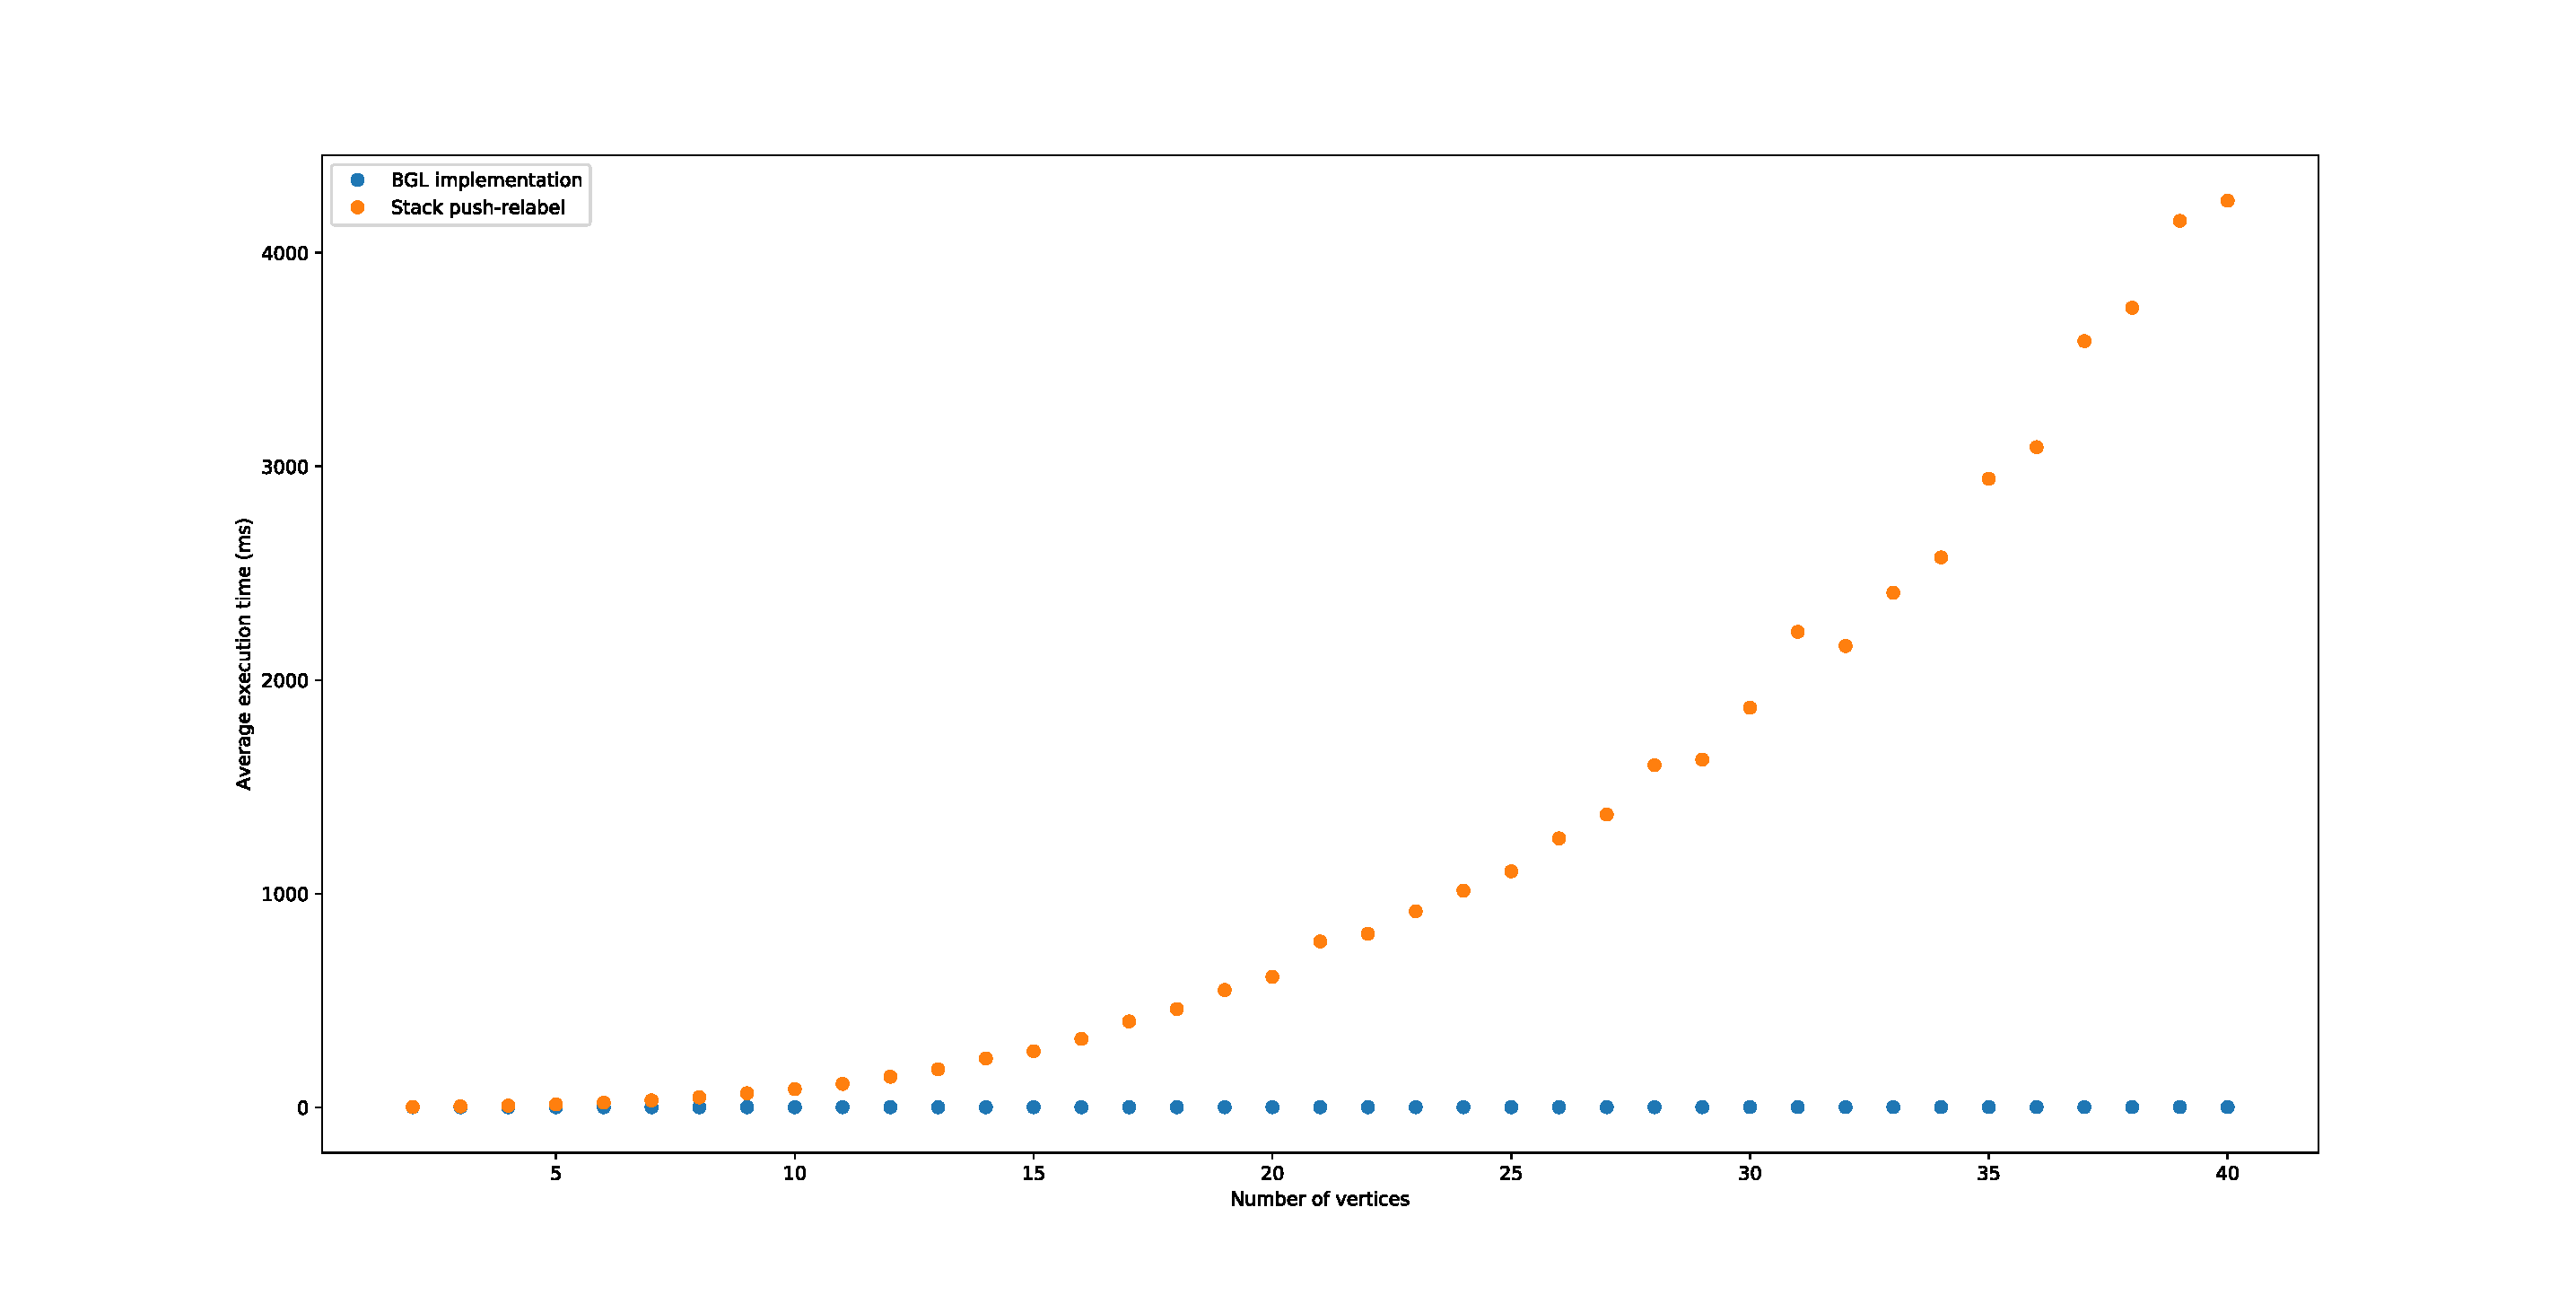
\includegraphics[width=1\textwidth]{time_vertices.pdf}
    \end{figure}

    \pause
    \begin{center}
        Execution time superlinear in the number of vertices...
    \end{center}
\end{frame}

\subsection{Number of edges}
\begin{frame}[fragile]{Execution time vs number of edges}
    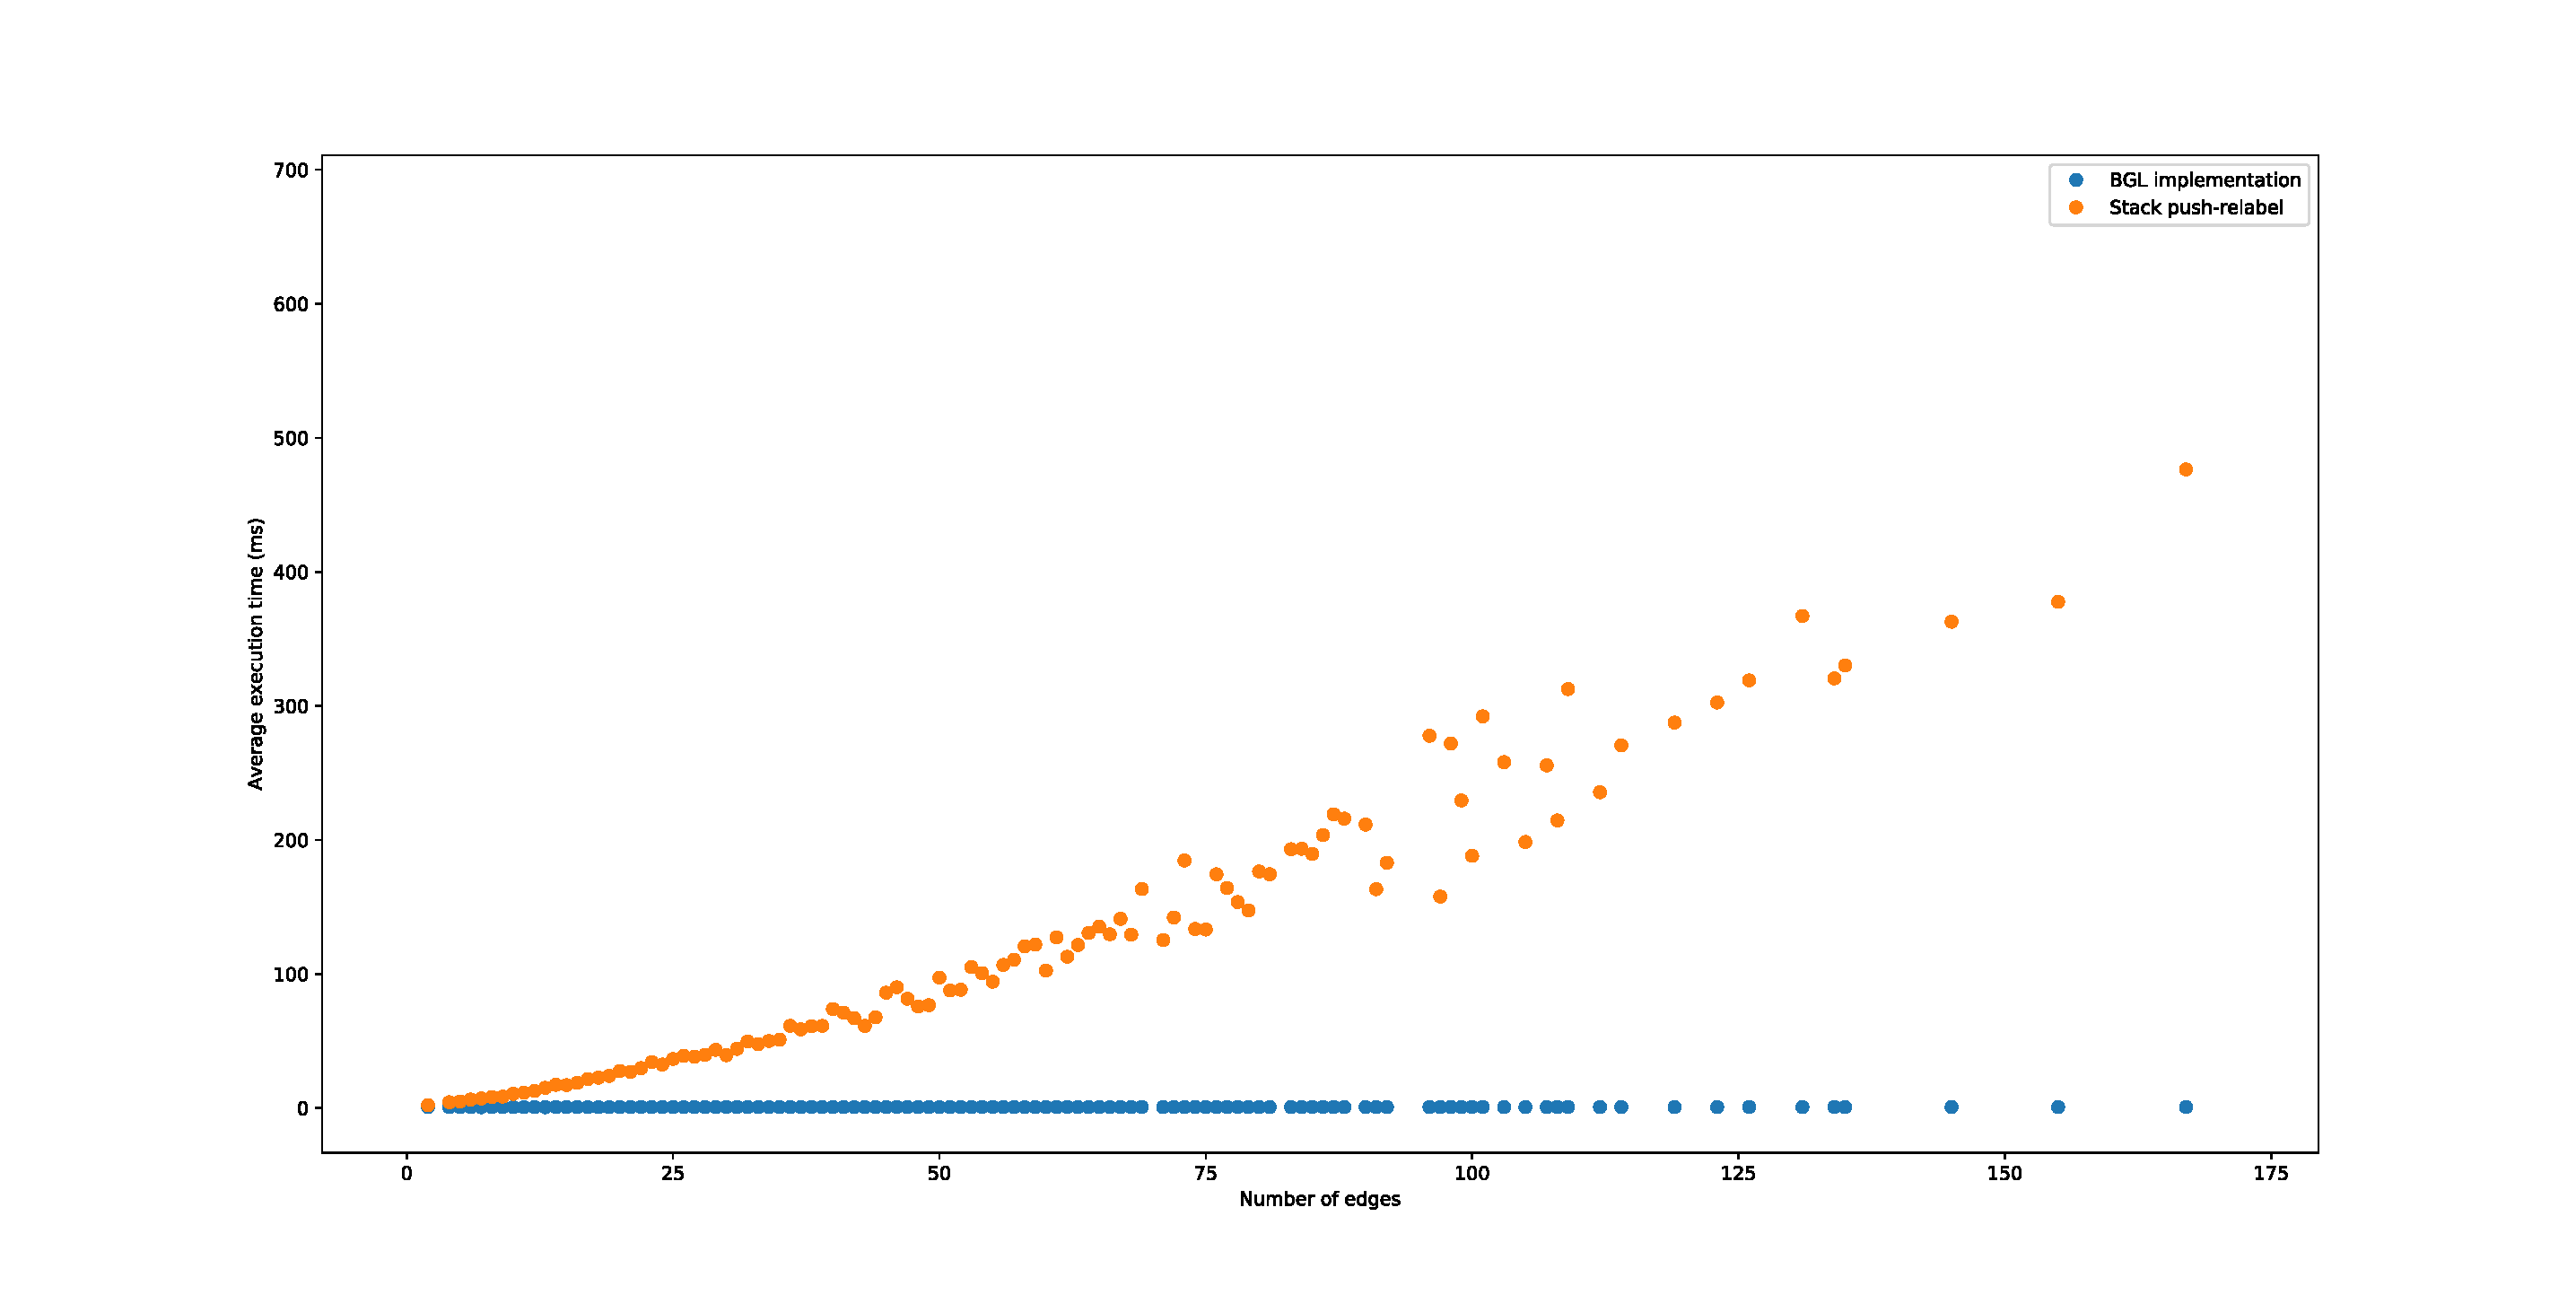
\includegraphics[width=1\textwidth]{time_edges.pdf}

    \pause
    \begin{center}
        ...and linear in the number of edges
    \end{center}
\end{frame}

\end{document}
